\section{Аналитический раздел}

\subsection{Постановка задачи}

В соответствии с заданием на курсовую работу необходимо разработать драйвер для изменения яркости и цветовой температуры дисплея с использованием USB-мыши.

Для достижения поставленной задачи необходимо:

\begin{enumerate}
	\item провести анализ USB-подсистемы Linux;
	\item провести анализ особенностей USB-устройства и формата передаваемых данных;
	\item разработать алгоритм работы драйвера;
	\item реализовать программный код драйвера;
	\item провести исследование результатов работы реализованного драйвера.
\end{enumerate}

\subsection{Особенности шины USB}

Устройства USB могут являться хабами, функциями или их комбинацией.

Хаб (hub) --- сетевой концентратор; обеспечивает дополнительные точки подключения устройств к шине.

Функции --- устройства, способные передавать или принимать данные или управляющую информацию по шине.
Функции USB предоставляют системе дополнительные возможности, например подключение акустической системы, мыши и т. п.

С точки зрения топологии, USB подсистема является не шиной, а деревом с одним корнем --- хостом (компьютером) с хост-контроллером, в который встроен корневой хаб (root hub) \cite{corbet2005linux}.
Хост-контроллер формирует запросы, а устройства посылают ответы.
Устройства никогда не отправляют информацию самостоятельно.
Запросы хост-контроллера имеют направление: IN --- хост отправляет запрос на прием данных, OUT --- хост отсылает данные устройству.
Схема USB топологии представлена на рисунке \ref{img:topology}.

\begin{figure}[!htb]\centering
	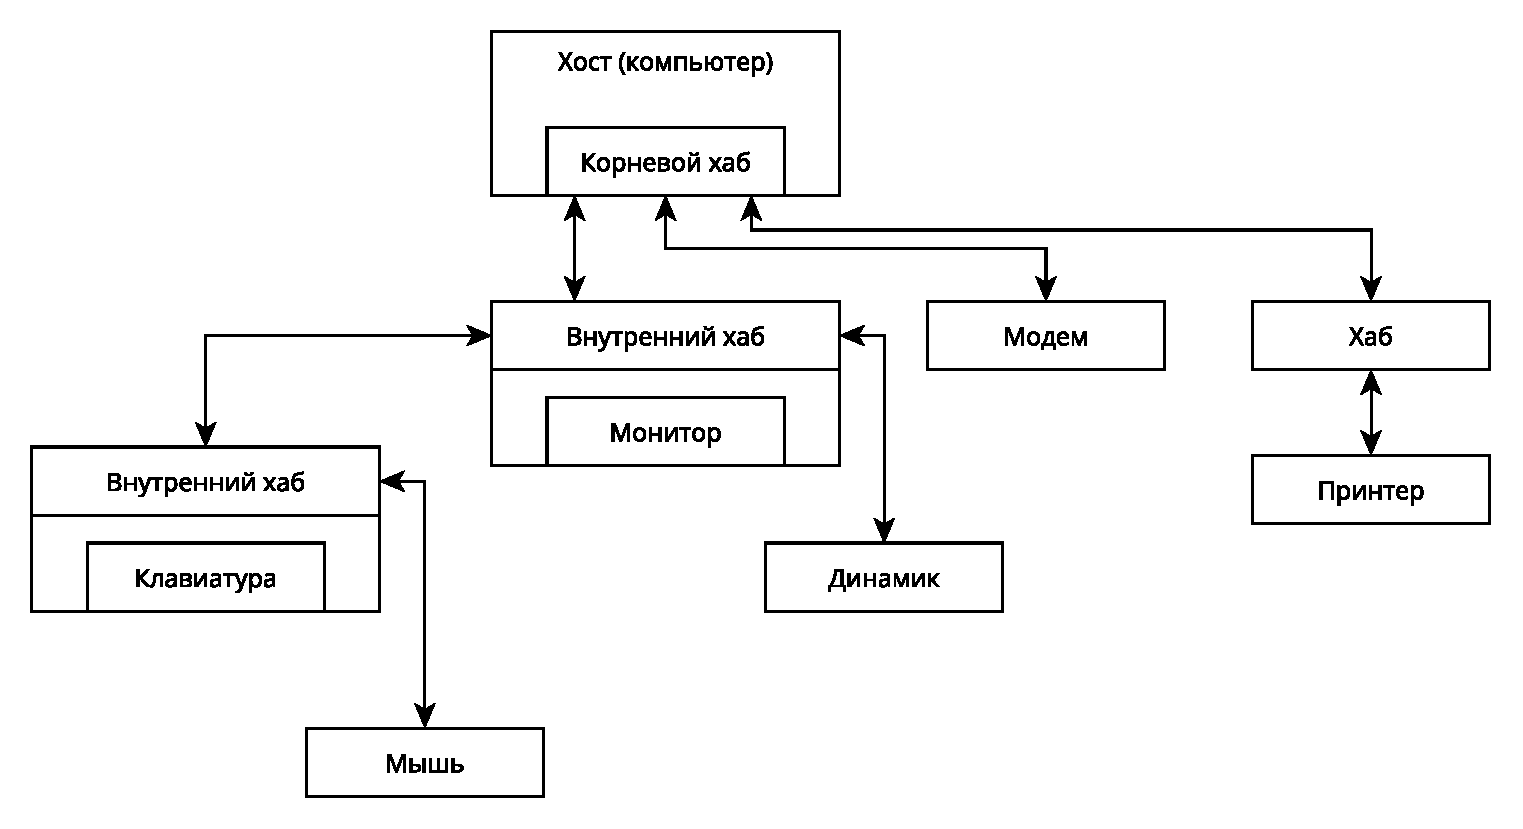
\includegraphics[width=0.9\textwidth]{../img/topology.pdf}
	\caption{USB топология}
	\label{img:topology}
\end{figure}

\newpage

Конечные точки (endpoints) --- базовые объекты связи интерфейсов USB.
Устройство может иметь до 16 конечных точек, нумерация начинается с 0 и заканчивается 15.
Каждая конечная точка может включать в себя два буфера (адреса): входной и выходной, то есть устройство может обладать 32 адресами конечных точек.
Каждая USB-функция должна содержать как минимум одну (нулевую) конечную точку с входным и выходным буфером.

Каналы (pipes) определяются хостом, они связаны с конечными точками функции.
В отличие от конечной точки, которая имеет физическую сущность, канал является всего лишь логической концепцией, правилом.
После установки канала, становится определенным и тип передачи данных, который он поддерживает.

Схема связи хоста и USB-интерфейсов представлена на рисунке \ref{img:endpoints}.

Архитектура (структура) USB-драйвера хоста представлена на рисунке \ref{img:general_driver}.

\begin{figure}[!htb]\centering
	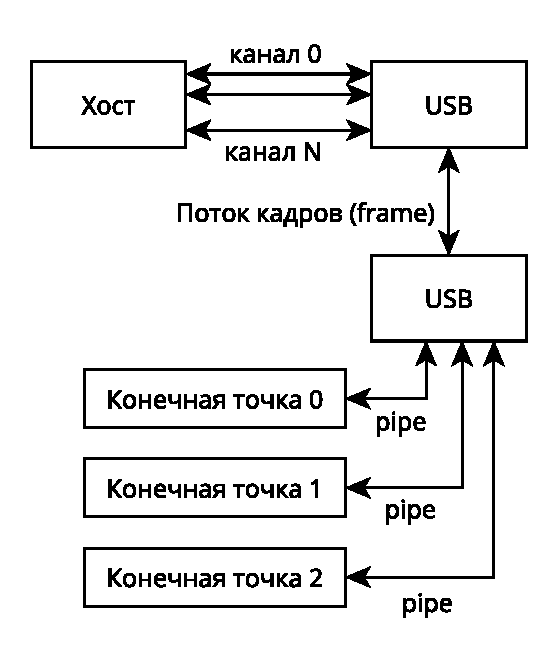
\includegraphics[width=0.5\textwidth]{../img/endpoints.pdf}
	\caption{Связь хоста и USB-интерфейсов (конечные точки, каналы)}
	\label{img:endpoints}
\end{figure}

\begin{figure}[!htb]\centering
	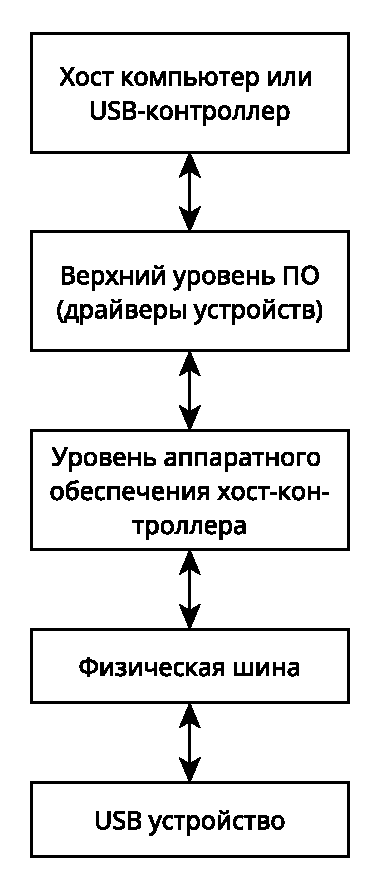
\includegraphics[width=0.295\textwidth]{../img/general_driver.pdf}
	\caption{Архитектура (структура) USB-драйвера хоста}
	\label{img:general_driver}
\end{figure}

\newpage

Задачей хоста является контроль данных, передающихся от устройства или на него.

Физическая шина --- <<USB кабель>>, который соединяет контроллер и периферию; состоит из четырех медных проводников (два отвечают за питание, другие два --- витая пара), то есть передача данных выполняется последовательно, а не параллельно.

В процессе передачи данных выполняются следующие действия:
\begin{enumerate}
	\item USB-устройство инициализирует передачу, используя функции интерфейса USB-драйвера, выдавая запросы драйверу;
	\item USB-драйвер отсылает запросы к модулю драйвера контроллера хоста (HCDM);
	\item HCDM делит запросы на отдельные транзакции, учитывая особенности шины и USB-устройства, и планирует транзакции по шине;
	\item хост-контроллер выполняет или завершает транзакцию (транзакция определяется шиной, устройство полностью зависимо).
\end{enumerate}

Передача осуществляется между буфером хоста и конечной точкой на USB-устройстве.
Шина является хост-ориентированной.
Хост-контроллер --- активная сторона шины.

Существует 4 типа передач:
\begin{enumerate}
	\item control --- передача является двунаправленной, предназначена для обмена с устройством короткими пакетами типа «вопрос-ответ», используется для отправки определенных общих команд на USB-устройство и позволяет программному обеспечению операционной системы прочитать информацию об устройстве (например, коды производителя и модели) (обычно осуществляется конечной точкой 0);
	\item isochronous --- изохронный канал имеет гарантированную пропускную способность (N пакетов за один период шины) и обеспечивает непрерывную передачу данных, подтверждение приема не требуется, для приложений реального времени;
	\item interrupt --- канал прерывания позволяет доставлять короткие пакеты без гарантии доставки и без подтверждений приема, но с гарантией времени доставки --- пакет будет доставлен не позже, чем через N миллисекунд (до 64 байт на полной скорости, до 8 байт на низкой скорости);
	\item bulk --- поточная или сплошная передача, используется устройствами, отправляющими и принимающими большое количество данных, но не имеющих определенную пропускную способность, имеется гарантия доставки каждого пакета; bulk пакеты имеют самый низкий приоритет, заполняют всю полосу пропускания шины.
\end{enumerate}

Для взаимодействия с USB-устройствами в ОС Linux предусмотрена структура URB.
Эта структура содержит необходимые для описания USB-запроса параметры, включая тип передачи данных, адрес назначения, буфер для данных, размер передачи и обратный вызов для обработки завершения запроса.
URB используется для всех типов USB-передач: control, bulk, interrupt и isochronous, что делает URB универсальным инструментом для взаимодействия с различными USB-устройствами.
Эта структура представлена на листинге \ref{lst:urb}.

\begin{longlisting}
	\singlespacing
	\caption{Структура urb}
	\label{lst:urb}
	\begin{minted}[frame=single,fontsize = \footnotesize, linenos, xleftmargin = 1.5em]{c}
struct urb {
  /* private: usb core and host controller only fields in the urb */
  struct kref kref;    /* reference count of the URB */
  int unlinked;      /* unlink error code */
  void *hcpriv;      /* private data for host controller */
  atomic_t use_count;    /* concurrent submissions counter */
  atomic_t reject;    /* submissions will fail */

  /* public: documented fields in the urb that can be used by drivers */
  struct list_head urb_list;  /* list head for use by the urb's
  * current owner */
  struct list_head anchor_list;  /* the URB may be anchored */
  struct usb_anchor *anchor;
  struct usb_device *dev;    /* (in) pointer to associated device */
  struct usb_host_endpoint *ep;  /* (internal) pointer to endpoint */
  unsigned int pipe;    /* (in) pipe information */
  unsigned int stream_id;    /* (in) stream ID */
  int status;      /* (return) non-ISO status */
  unsigned int transfer_flags;  /* (in) URB_SHORT_NOT_OK | ...*/
  void *transfer_buffer;    /* (in) associated data buffer */
  dma_addr_t transfer_dma;  /* (in) dma addr for transfer_buffer */
  struct scatterlist *sg;    /* (in) scatter gather buffer list */
  int num_mapped_sgs;    /* (internal) mapped sg entries */
  int num_sgs;      /* (in) number of entries in the sg list */
  u32 transfer_buffer_length;  /* (in) data buffer length */
  u32 actual_length;    /* (return) actual transfer length */
  unsigned char *setup_packet;  /* (in) setup packet (control only) */
  dma_addr_t setup_dma;    /* (in) dma addr for setup_packet */
  int start_frame;    /* (modify) start frame (ISO) */
  int number_of_packets;    /* (in) number of ISO packets */
  int interval;      /* (modify) transfer interval
  * (INT/ISO) */
  int error_count;    /* (return) number of ISO errors */
  void *context;      /* (in) context for completion */
  usb_complete_t complete;  /* (in) completion routine */
  struct usb_iso_packet_descriptor iso_frame_desc[];
  /* (in) ISO ONLY */
};
	\end{minted}
\end{longlisting}

\subsection{USB драйвер}

В Linux имеются драйверы трех типов:
\begin{enumerate}
	\item низкого уровня --- пишутся разработчиками устройств;
	\item верхнего уровня --- реализованы как загружаемые модули ядра;
	\item смешанного уровня --- код поделен между ядром и специальной утилитой, управляющей устройством.
\end{enumerate}

Схема взаимодействия прикладных программ с аппаратной частью компьютера: устройство $\Leftrightarrow$ ядро $\Leftrightarrow$ специальный файл устройства $\Leftrightarrow$ программа пользователя.

Драйвер ОС Linux представляет собой загружаемый модуль ядра, который определяет точки входа для работы с устройством.
Инициализируются и заполняются следующие структуры:

\begin{itemize}
	\item структура \texttt{usb\_driver}, представленная на листинге \ref{lst:usb_driver} и описывающая тип устройства, имя, точки входа, коды производителя и модели;
	\item структура \texttt{usb\_class\_driver}, представленная на листинге \ref{lst:usb_class_driver} и описывающая создаваемый специальный файл (блочный) в директории \texttt{/dev/};
	\item структура, содержащая данные для работы драйвера с конкретным USB-устройством.
\end{itemize}

\begin{longlisting}
	\singlespacing
	\caption{Структура usb\_driver}
	\label{lst:usb_driver}
	\begin{minted}[frame=single,fontsize = \footnotesize, linenos, xleftmargin = 1.5em]{c}
struct usb_driver {
  const char *name;	
  int (*probe) (struct usb_interface *intf, 
  	      const struct usb_device_id *id);
  void (*disconnect) (struct usb_interface *intf);
  int (*unlocked_ioctl) (struct usb_interface *intf, unsigned int code,
                         void *buf);
  int (*suspend) (struct usb_interface *intf, pm_message_t message);
  int (*resume) (struct usb_interface *intf);
  int (*reset_resume)(struct usb_interface *intf);
  int (*pre_reset)(struct usb_interface *intf);
  int (*post_reset)(struct usb_interface *intf);
  void (*shutdown)(struct usb_interface *intf);
  const struct usb_device_id *id_table;
  const struct attribute_group **dev_groups;
  struct usb_dynids dynids;
  struct device_driver driver;
  unsigned int no_dynamic_id:1;
  unsigned int supports_autosuspend:1;
  unsigned int disable_hub_initiated_lpm:1;
  unsigned int soft_unbind:1;
};
	\end{minted}
\end{longlisting}

Функции, являющиеся основными точками входа драйвера, описаны далее.

\begin{itemize}
	\item probe() --- функция, вызываемая при подключении устройства; заполняет те поля структуры, описывающей конкретное USB-устройство, которые можно получить непосредственно при его подключении (USB-интерфейс устройства, адрес его конечной точки, размер буфера для передачи данных); далее создается URB с соответствующими параметрами и файл в директории /dev/; URB подтверждается, после чего хост начинает отправлять периодические запросы на получение данных с устройства (тип передачи interrupt transfer).
	
	\item disconnect() --- функция, вызываемая при отключении устройства; удаляет соответствующий файл из директории /dev/.
	
	\item read() --- переопределенная функция чтения из файла устройства; упаковывает данные ввода из 64-байтового пакета данных в 4-байтовый массив и копирует его в пространство пользователя.
	
	\item init() --- функция инициализации модуля; регистрирует данный тип устройства в системе.
	
	\item exit() --- функция выгрузки модуля; выгружает данный тип устройства из системы.
\end{itemize}

\begin{longlisting}
	\singlespacing
	\caption{Структура usb\_class\_driver}
	\label{lst:usb_class_driver}
	\begin{minted}[frame=single,fontsize = \footnotesize, linenos, xleftmargin = 1.5em]{c}
struct usb_class_driver {
  char *name;
  char *(*devnode)(const struct device *dev, umode_t *mode);
  const struct file_operations *fops;
  int minor_base;
};
	\end{minted}
\end{longlisting}

\subsection{Особенности USB-мыши и разрабатываемого ПО}

Для определения формата передаваемых устройством данных, а также некоторых его параметров была использована программа Wireshark.
Данное ПО позволяет перехватить трафик между уже существующим HID-драйвером и устройством.

В результате анализа результатов работы программы Wireshark выяснено, что
\begin{itemize}
	\item необработанные данные устройства представляют из себя пакет размером 64 байта, из них 4 байта используются для передачи пользовательского ввода;
	\item 0-й байт --- направление движения колесика (0 --- не двигается, 1 --- вниз, 255 --- вверх);
	\item 1-й байт --- смещение мыши по координатам оси X;
	\item 2-й байт --- смещение мыши по координатам оси Y;
	\item 3-й байт --- состояние клавиш мыши (левой --- нулевой бит, правой --- первый бит, средней --- второй бит);
	\item USB-мышь имеет одну конечную точку с номером 0 по адресу 80h.
\end{itemize}

Схема поля data пакета, передаваемого с устройства, представлена на рисунке \ref{img:data}.

\begin{figure}[!htb]\centering
	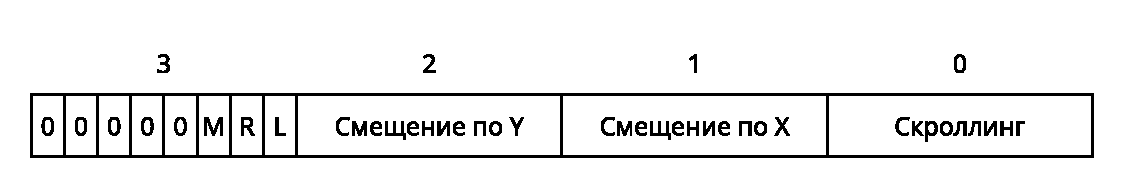
\includegraphics[width=0.9\textwidth]{../img/data.pdf}
	\caption{Схема поля data пакета, передаваемого с устройства}
	\label{img:data}
\end{figure}

Изменение яркости дисплея осуществляется двумя способами:

\begin{enumerate}
	\item с использованием функции ядра \texttt{intel\_backlight\_set\_acpi};
	\item с использованием файловой системы sysfs, осуществляя чтение из и запись в файл \texttt{/sys/class/backlight/intel\_backlight/brightness}.
\end{enumerate}

Изменение цветовой температуры дисплея осуществляется в пространстве пользователя посредством изменения значения переменной в файле, содержащем настройки GNOME.
Это выполняется при помощи утилиты gsettings, пример использования представлен на листинге \ref{lst:gsettings}.

\begin{longlisting}
	\caption{Использование утилиты gsettings}
	\label{lst:gsettings}
	\begin{minted}[frame=single,fontsize=\scriptsize, linenos, xleftmargin = 1.5em]{sh}
gsettings get org.gnome.settings-daemon.plugins.color night-light-temperature
	\end{minted}
\end{longlisting}

Поскольку был найден только такой способ изменения цветовой температуры дисплея, было принято решение изменять яркость дисплея с использованием файловой системы sysfs.

Таким образом, в качестве типа разрабатываемого программного обеспечения выбраны драйвер, реализованный в виде загружаемого модуля ядра, и демон, который осуществляет чтение данных из специального файла устройства и изменение яркости, теплоты дисплея.

\subsection*{Выводы}

В результате проведенного анализа были сделаны следующие выводы:

\begin{itemize}
	\item для изменения поведения USB-мыши необходимо разработать USB-драйвер, осуществляющий запись данных устройства в специальный файл устройства, и демон, который считывает эти данные и выполняет дальнейшие изменения в системе;
	\item для изменения яркости необходимо взаимодействовать с файловой системой sysfs;
	\item для изменения цветовой температуры необходимо использовать утилиту gsettings;
	\item для определения вида взаимодействия устройства и системы будет использована структура URB.
\end{itemize}